\begin{name}
	{\tenchude}
	{\tendethi}
	{\tentruong}
	{\thoigian}
\end{name}
\TN
\Opensolutionfile{ans}[ans/ans\currfilebase]

\begin{ex}%[2D1N4-1]%[Dự án đề kiểm tra Toán GHKI NH 24-25- Phan Anh]%[THPT Phạm Văn Sáng - Tp HCM]
	Đường thẳng nào dưới đây là tiệm cận ngang của đồ thị hàm số $y=\dfrac{-x+1}{2x+1}$?
	\choice
	{\True $y=-\dfrac{1}{2}$}
	{$y=1$}
	{$y=-1$}
	{$y=-2$}
	\loigiai{Ta có $\lim\limits_{x\to\pm\infty}y=\lim\limits_{x\to\pm\infty}\dfrac{-x+1}{2x+1}=-\dfrac{1}{2}$.\\
		Suy ra đồ thị hàm số nhận $y=-\dfrac{1}{2}$ làm tiệm cận ngang.}
\end{ex}
\begin{ex}%[2D1N2-1]%[Dự án đề kiểm tra Toán GHKI NH 24-25- Phan Anh]%[THPT Phạm Văn Sáng - Tp HCM]
	Hàm số $y=\dfrac{2x-3}{x+1}$ có bao nhiêu điểm cực trị?
	\choice
	{\True $0$}
	{$3$}
	{$2$}
	{$1$}
	\loigiai{Ta có $y'=\dfrac{5}{(x+1)^2}>0$, $\forall x\in\mathbb{R}\setminus\{-1\}$ nên hàm số không có điểm cực trị.}
\end{ex}
\begin{ex}%[2D1N3-1]%[Dự án đề kiểm tra Toán GHKI NH 24-25- Phan Anh]%[THPT Phạm Văn Sáng - Tp HCM]
	\immini[thm]{Cho hàm số $f(x)$ có đồ thị trên đoạn $[-3;3]$ như hình vẽ. Tổng giá trị lớn nhất và giá trị nhỏ nhất của hàm số $f(x)$ trên đoạn $[-3;3]$ là
		\choice
		{\True $2$}
		{$3$}
		{$4$}
		{$-2$}
	}{\begin{tikzpicture}[>=stealth,line join=round,line cap=round,font=\footnotesize,scale=0.75]
			\draw[->] (-4,0)--(4,0) node[right] {$x$};
			\draw[->] (0,-3)--(0,5) node[above] {$y$};
			\draw
			[smooth,domain=-3:-1,samples=100]plot(\x,{-1.25*(\x)^2-2.5*(\x)+1.75})
			[smooth,domain=-1:1,samples=100]plot(\x,{-2*(\x)^3+1})
			(1,-1)--(3,4);
			\draw[dashed] (-3,0)--(-3,-2)--(0,-2) (-1,0)--(-1,3)--(0,3) (1,0)--(1,-1)--(0,-1) (3,0)--(3,4)--(0,4);
			\fill (0,0)node[shift={(135:2.5mm)}]{\footnotesize{$O$}}circle(1.2pt) (1,0)node[above]{\footnotesize{$1$}}circle(1.2pt) (-1,0)node[below]{\footnotesize{$-1$}}circle(1.2pt) (-3,0)node[above]{\footnotesize{$-3$}}circle(1.2pt) (3,0)node[below]{\footnotesize{$3$}}circle(1.2pt) (0,3)node[right]{\footnotesize{$3$}}circle(1.2pt) (0,4)node[left]{\footnotesize{$4$}}circle(1.2pt) (0,-1)node[left]{\footnotesize{$-1$}}circle(1.2pt) (0,-2)node[right]{\footnotesize{$-2$}}circle(1.2pt);
		\end{tikzpicture}}
	\loigiai{Dựa vào hình vẽ, giá trị lớn nhất và giá trị nhỏ nhất của hàm số trên $[-3;3]$ lần lượt là $4$ và $-2$.\\
		Suy ra tổng giá trị lớn nhất và giá trị nhỏ nhất của hàm số $f(x)$ trên đoạn $[-3;3]$ là $T=4-2=2$.}
\end{ex}
\begin{ex}%[2D1H2-1]%[Dự án đề kiểm tra Toán GHKI NH 24-25- Phan Anh]%[THPT Phạm Văn Sáng - Tp HCM]
	Hàm số $f(x)=x^3-3x^2-9x+1$ đạt cực đại tại điểm
	\choice
	{$x=-3$}
	{\True $x=-1$}
	{$x=1$}
	{$x=3$}
	\loigiai{Ta có $y'=3x^2-6x-9$.\\
		$y'=0\Leftrightarrow3x^2-6x-9=0\Leftrightarrow\hoac{&x=-1\\&x=3.}$\\
		Bảng biến thiên của hàm số như hình vẽ
		\begin{center}
			
\begin{tikzpicture}[scale=1, font=\footnotesize, line join=round, line cap=round, >=stealth]
				\tkzTabInit[nocadre=false, lgt=1.2, espcl=2.8, deltacl=0.6]
				{$x$/0.6, $y'$/0.6,$y$/2}
				{$-\infty$,$-1$,$3$,$+\infty$}
				\tkzTabLine{,+,0,-,0,+,}
				\tkzTabVar{-/$ $,+/$ $,-/$ $,+/$ $}
			\end{tikzpicture}
		\end{center}
		Dựa vào bảng biến thiên, hàm số đạt cực đại tại điểm $x=-1$.}
\end{ex}
\begin{ex}%[2D1N5-1]%[Dự án đề kiểm tra Toán GHKI NH 24-25- Phan Anh]%[THPT Phạm Văn Sáng - Tp HCM]
	\immini[thm]{Đường cong trong hình vẽ là đồ thị của hàm số nào bên dưới?
		\choice[2]
		{$y=x^3-3x^2+2$}
		{$y=\dfrac{x+1}{x-1}$}
		{\True $y=\dfrac{x-1}{x+1}$}
		{$y=x^4-2x^2-1$}}
	{\begin{tikzpicture}[>=stealth,line join=round,line cap=round,font=\footnotesize,scale=0.5]
			\draw[->] (-5,0)--(5,0) node[right] {$x$};
			\draw[->] (0,-4)--(0,6) node[above] {$y$};
			\draw
			[smooth,domain=-5:-1.4,samples=100]plot(\x,{(\x-1)/(\x+1)})
			[smooth,domain=-0.6:5,samples=100]plot(\x,{(\x-1)/(\x+1)})
			(-1,-4)--(-1,6) (-5,1)--(5,1);
			\fill (0,0)node[shift={(45:2.5mm)}]{\footnotesize{$O$}}circle(1.2pt) (-1,0)node[below left]{\footnotesize{$-1$}}circle(1.2pt) (0,1)node[above right]{\footnotesize{$1$}}circle(1.2pt);
		\end{tikzpicture}}
	\loigiai{Dựa vào hình vẽ, ta thấy đây là đồ thị hàm số nhận $x=-1$ làm tiệm cận đứng nên hàm số thỏa mãn là $y=\dfrac{x-1}{x+1}$.}
\end{ex}
\begin{ex}%[2D1H1-1]%[Dự án đề kiểm tra Toán GHKI NH 24-25- Phan Anh]%[THPT Phạm Văn Sáng - Tp HCM]
	Hàm số $y=-x^3+3x^2+2$ đồng biến trên khoảng nào dưới đây?
	\choice
	{$(0;4)$}
	{$(2;+\infty)$}
	{\True $(0;2)$}
	{$(-\infty;0)$}
	\loigiai{Ta có $y'=-3x^2+6x$, hàm số đồng biến khi
		\[y'\ge0\Leftrightarrow-3x^2+6x\ge0\Leftrightarrow0\le x\le2.\]
		Vậy hàm số đồng biến trên khoảng $(0;2)$.}
\end{ex}
\begin{ex}%[2D1H4-1]%[Dự án đề kiểm tra Toán GHKI NH 24-25- Phan Anh]%[THPT Phạm Văn Sáng - Tp HCM]
	Đường thẳng $x=2$ là tiệm cận đứng của đồ thị hàm số nào dưới đây?
	\choice
	{$y=\dfrac{1+x}{1-2x}$}
	{\True $y=\dfrac{-2x+2}{x-2}$}
	{$y=\dfrac{2x+3}{2+x}$}
	{$y=\dfrac{-2x+2}{1-x}$}
	\loigiai{Xét hàm số $y=\dfrac{-2x+2}{x-2}$, có $\lim\limits_{x\to2^+}y=\lim\limits_{x\to2^+}\dfrac{-2x+2}{x-2}=-\infty$.\\
		Suy ra đồ thị của hàm số $y=\dfrac{-2x+2}{x-2}$ nhận $x=2$ làm tiệm cận đứng.}
\end{ex}
\begin{ex}%[2D1N5-1]%[Dự án đề kiểm tra Toán GHKI NH 24-25- Phan Anh]%[THPT Phạm Văn Sáng - Tp HCM]
	\immini[thm]{Đồ thị hàm số nào sau đây có hình dạng như hình vẽ bên?
		\choice[2]
		{$y=-x^3+3x$}
		{$y=-x^3+3x^2$}
		{\True $y=x^3-3x^2$}
		{$y=x^3-3x+1$}}
	{\begin{tikzpicture}[>=stealth,line join=round,line cap=round,font=\footnotesize,scale=0.65,xscale=1.2]
			\draw[->] (-2,0)--(4,0) node[right] {$x$};
			\draw[->] (0,-5)--(0,1) node[above] {$y$};
			\draw [smooth,domain=-1.1:3.1,samples=100]plot(\x,{(\x)^3-3*(\x)^2});
			\draw[dashed](2,0)--(2,-4)--(0,-4);
			\fill (0,0)node[shift={(135:2.5mm)}]{\footnotesize{$O$}}circle(1.2pt) (2,0)node[above]{\footnotesize{$2$}}circle(1.2pt) (0,-4)node[left]{\footnotesize{$-4$}}circle(1.2pt);
		\end{tikzpicture}}
	\loigiai{Đường cong trong hình vẽ là đồ thị của hàm số $y=ax^3+bx^2+cx+d$ với $a>0$.\\
		Ngoài ra đồ thị hàm số còn đi qua điểm $(0;0)$ nên chỉ có hàm số $y=x^3-3x^2$ thỏa mãn.}
\end{ex}
\begin{ex}%[2D1N1-2]%[Dự án đề kiểm tra Toán GHKI NH 24-25- Phan Anh]%[THPT Phạm Văn Sáng - Tp HCM]
	Cho hàm số $f(x)$ có bảng biên thiên như bên dưới
	\begin{center}
		
\begin{tikzpicture}[scale=1, font=\footnotesize, line join=round, line cap=round, >=stealth]
			\tkzTabInit[nocadre=false, lgt=1.2, espcl=2.8, deltacl=0.6]
			{$x$/0.6, $f'(x)$/0.6,$f(x)$/2}
			{$-\infty$,$0$,$2$,$+\infty$}
			\tkzTabLine{,+,0,-,0,+,}
			\tkzTabVar{-/$-\infty$,+/$1$,-/$-3$,+/$+\infty$}
		\end{tikzpicture}
	\end{center}
	Hàm số đã cho nghịch biến trên khoảng nào dưới đây?
	\choice
	{$(-3;1)$}
	{$(-\infty;1)$}
	{$(2;+\infty)$}
	{\True $(0;2)$}
	\loigiai{Dựa vào bảng biến thiên, hàm số nghịch biến trên khoảng $(0;2)$.}
\end{ex}
\begin{ex}%[2D1H3-1]%[Dự án đề kiểm tra Toán GHKI NH 24-25- Phan Anh]%[THPT Phạm Văn Sáng - Tp HCM]
	Giá trị nhỏ nhất của hàm số $y=x^2-2x+3$ trên đoạn $[2;4]$ là
	\choice
	{$-1$}
	{$2$}
	{\True $3$}
	{$1$}
	\loigiai{Ta có $y'=2x-2>0$, $\forall x\in[2;4]$.\\
		Suy ra hàm số đồng biến trên $[2;4]$, vậy giá trị nhỏ nhất của hàm số trên đoạn $[2;4]$ là $y(2)=3$.}
\end{ex}
\begin{ex}%[2D1N5-1]%[Dự án đề kiểm tra Toán GHKI NH 24-25- Phan Anh]%[THPT Phạm Văn Sáng - Tp HCM]
	\immini[thm]{Đồ thị hàm số nào sau đây có hình dạng như hình vẽ bên dưới?
		\choice[2]
		{$y=\dfrac{x^2+x-1}{x-2}$}
		{$y=\dfrac{x^2-x+1}{x+2}$}
		{$y=\dfrac{x^2-2x-1}{x-2}$}
		{\True $y=\dfrac{x^2-x-1}{x-2}$}}
	{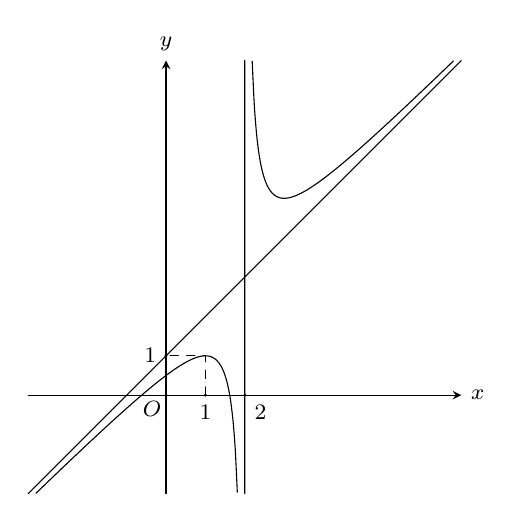
\begin{tikzpicture}[>=stealth,line join=round,line cap=round,font=\footnotesize,scale=0.5]
			\draw[->] (-3.5,0)--(7.5,0) node[right] {$x$};
			\draw[->] (0,-2.5)--(0,8.5) node[above] {$y$};
			\draw
			[smooth,domain=-3.3:1.811,samples=100]plot(\x,{((\x)^2-(\x)-1)/(\x-2)})
			[smooth,domain=2.189:7.3,samples=100]plot(\x,{((\x)^2-(\x)-1)/(\x-2)})
			[smooth,domain=-3.5:7.5,samples=100]plot(\x,{\x+1})
			(2,-2.5)--(2,8.5)
			;
			\draw[dashed] (1,0)--(1,1)--(0,1);
			\fill (0,0)node[shift={(-135:2.5mm)}]{\footnotesize{$O$}}circle(1.2pt) (1,0)node[below]{\footnotesize{$1$}}circle(1.2pt) (2,0)node[below right]{\footnotesize{$2$}}circle(1.2pt) (0,1)node[left]{\footnotesize{$1$}}circle(1.2pt);
		\end{tikzpicture}}
	\loigiai{Đồ thị hàm số trong hình vẽ đi qua điểm $(1;1)$, nhận $x=2$ làm tiệm cận đứng.\\
		Suy ra chỉ có hàm số $y=\dfrac{x^2-x-1}{x-2}$ thỏa mãn.}
\end{ex}
\begin{ex}%[2D1N5-1]%[Dự án đề kiểm tra Toán GHKI NH 24-25- Phan Anh]%[THPT Phạm Văn Sáng - Tp HCM]
	\immini[thm]{Đường cong ở hình bên là đồ thị của hàm số nào?
		\choice[2]
		{$y=x^3-x^2-4$}
		{$y=-x^3+6x-4$}
		{$y=x^3-2x-4$}
		{\True $y=-x^3+3x^2-4$}}
	{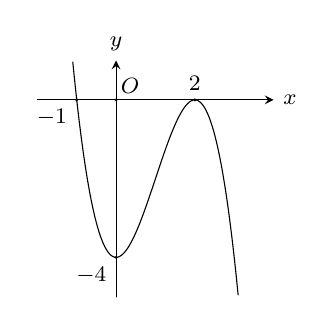
\begin{tikzpicture}[>=stealth,line join=round,line cap=round,font=\footnotesize,scale=0.5]
			\draw[->] (-2,0)--(4,0) node[right] {$x$};
			\draw[->] (0,-5)--(0,1) node[above] {$y$};
			\draw [smooth,domain=-1.1:3.1,samples=100]plot(\x,{-(\x)^3+3*(\x)^2-4});
			\fill (0,0)node[shift={(45:2.5mm)}]{\footnotesize{$O$}}circle(1.2pt) (2,0)node[above]{\footnotesize{$2$}}circle(1.2pt) (-1,0)node[below left]{\footnotesize{$-1$}}circle(1.2pt) (0,-4)node[below left]{\footnotesize{$-4$}}circle(1.2pt);
		\end{tikzpicture}}
	\loigiai{Đường cong trong hình vẽ là đồ thị của hàm số bậc ba $y=ax^3+bx^2+cx+d$ với $a<0$.\\
		Đồng thời đồ thị đi qua điểm $(-1;0)$ và $(2;0)$ nên chỉ có hàm số $y=-x^3+3x^2-4$ thỏa mãn.}
\end{ex}

\TNTF

\begin{ex}%[2D1H4-1]%[Dự án đề kiểm tra Toán GHKI NH 24-25- Phan Anh]%[THPT Phạm Văn Sáng - Tp HCM]
	Cho hàm số $y=\dfrac{2x^2-2x+2}{-x+1}$ có đồ thị $(C)$.
	\choiceTF
	{Hàm số đạt cực tiểu tại $x=2$}
	{Hàm số nghịch biến trên khoảng $(-\infty;0)\cup(2;+\infty)$}
	{\True Đồ thị $(C)$ có tiệm cận xiên là đường thẳng $2x+y=0$}
	{Giá trị nhỏ nhất của hàm số trên đoạn $\left[\dfrac{3}{2};\dfrac{5}{2}\right]$ bằng $-\dfrac{19}{3}$}
	\loigiai{Tập xác định là $\mathscr{D}=\mathbb{R}\setminus\{1\}$.\\
		Ta có $y'=\dfrac{-2x^2+4x}{(-x+1)^2}$, $y'=0\Leftrightarrow\hoac{&x=0\\&x=2.}$\\
		Bảng biến thiên của hàm số như hình vẽ
		\begin{center}
			\begin{tikzpicture}[scale=1, font=\footnotesize, line join=round, line cap=round, >=stealth]
				\tkzTabInit[nocadre=false, lgt=1.2, espcl=2.8, deltacl=0.6]
				{$x$/0.6, $y'$/0.6,$y$/2.4}
				{$-\infty$,$0$,$1$,$2$,$+\infty$}
				\tkzTabLine{,-,0,+,d,+,0,-,}
				\tkzTabVar{+/$ $,-/$ $,+D-/$ $/$ $,+/$ $,-/$ $}
				\tkzTabVal[draw]{3}{4}{0.5}{$\tfrac{3}{2}$}{$-7$}
				\tkzTabVal[draw]{4}{5}{0.5}{$\tfrac{5}{2}$}{$-\dfrac{19}{3}$}
			\end{tikzpicture}
		\end{center}
		\begin{itemchoice}
			\itemch Dựa vào bảng biến thiên, hàm số đạt cực tiểu tại $x=0$
			\itemch Dựa vào bảng biến thiên, hàm số nghịch biến trên khoảng $(-\infty;0)$ và $(2;+\infty)$.
			\itemch Ta có $y=\dfrac{2x^2-2x+2}{-x+1}=-2x+\dfrac{2}{-x+1}$.\\
			Suy ra $\lim\limits_{x\to\pm\infty}\left(y+2x\right)=\lim\limits_{x\to\pm\infty}\dfrac{2}{-x+1}=0$ nên $2x+y=0$ là tiệm cận xiên của đồ thị $(C)$.
			\itemch Dựa vào bảng biến thiên, giá trị nhỏ nhất của hàm số trên đoạn $\left[\dfrac{3}{2};\dfrac{5}{2}\right]$ là $y\left(\dfrac{3}{2}\right)=-7$.
		\end{itemchoice}}
\end{ex}

\begin{ex}%[2D1V3-6]%[Dự án đề kiểm tra Toán GHKI NH 24-25- Phan Anh]%[THPT Phạm Văn Sáng - Tp HCM]
	Người ta bơm xăng vào bình xăng của một xe ô tô, biết rằng thể tích $V$\,(lít) của lượng xăng trong bình xăng được tính theo thời gian bơm xăng $t$\,(phút) được cho bởi công thức
	\[V(t)=300\left(t^2-t^3\right)+4\text{ với }0\le t\le0{,}5.\]
	Gọi $V'(t)$ là tốc độ tăng thể tích tại thời điểm $t$, với $0\le t\le0{,}5$.
	\choiceTF
	{Lượng xăng ban đầu trong bình là $1$\,lít}
	{$V'(t)=300\left(2t-3t^2\right)+4$, với $0\le t\le0{,}5$}
	{Xăng chảy vào bình xăng vào thời điểm ở giây thứ $30$ có tốc độ tăng thể tích là lớn nhất}
	{\True Lượng xăng lớn nhất bơm vào bình xăng là $41{,}5$\,lít}
	\loigiai{
		\begin{itemchoice}
			\itemch Lượng xăng ban đầu trong bình là $V(0)=4$\,lít.
			\itemch Ta có $V'(t)=300\left(2t-3t^2\right)$, với $0\le t\le0{,}5$.
			\itemch Ta có $V''(t)=300(2-6t)$,  $V''(t)=0\Leftrightarrow t=\dfrac{1}{6}$.\\
			Bảng biến thiên của $V'(t)$ như hình vẽ
			\begin{center}
				\begin{tikzpicture}[scale=1 line join=round, line cap=round, >=stealth]
					\tkzTabInit[nocadre=false, lgt=1.2, espcl=2.8, deltacl=0.6]
					{$x$/0.6, $V''(t)$/0.6,$V'(t)$/2}
					{$0$,$\dfrac{1}{6}$,$0{,}5$}
					\tkzTabLine{,+,0,-,}
					\tkzTabVar{-/$ $,+/$ $,-/$ $}
				\end{tikzpicture}
			\end{center}
			Vậy tại thời điểm $t=\dfrac{1}{6}$\,(phút)$=10$\,(giây) thì tốc độ tăng thể tích là lớn nhất.
			\itemch Ta có $V'(t)=300t(2-3t)>0$, $\forall t\in[0;0{,}5]$ nên $V(t)$ đồng biến trên đoạn $[0;0{,}5]$.\\
			Suy ra lượng xăng lớn nhất bơm vào bình xăng là $V(0{,}5)=41{,}5$\,lít.
		\end{itemchoice}
	}
\end{ex}

\begin{ex}%[2D1N2-2]%[Dự án đề kiểm tra Toán GHKI NH 24-25- Phan Anh]%[THPT Phạm Văn Sáng - Tp HCM]
	Cho hàm số $y=f(x)$ có bảng biến thiên như hình vẽ bên dưới
	\begin{center}
		
\begin{tikzpicture}[scale=1, line join=round, line cap=round, >=stealth]
			\tkzTabInit[nocadre=false, lgt=1.2, espcl=2.8, deltacl=0.6]
			{$x$/0.6, $y'$/0.6,$y$/2}
			{$-\infty$,$-2$,$0$,$2$,$+\infty$}
			\tkzTabLine{,-,0,+,d,+,0,-,}
			\tkzTabVar{+/$\infty$,-/$-1$,+D-/$2$/$-\infty$,+/$2$,-/$-\infty$}
		\end{tikzpicture}
	\end{center}
	\choiceTF
	{\True Giá trị cực đại của hàm số bằng $2$}
	{\True Giá trị cực tiểu của hàm số bằng $-1$}
	{Hàm số đạt cực đại tại $x=0$ và $x=1$}
	{\True Hàm số đạt cực tiểu tại $x=-2$}
	\loigiai{
		\begin{itemchoice}
			\itemch Giá trị cực đại của hàm số bằng $2$.
			\itemch Giá trị cực tiểu của hàm số bằng $-1$
			\itemch Hàm số đạt cực đại tại $x=2$.
			\itemch Hàm số đạt cực tiểu tại $x=-2$.
		\end{itemchoice}
	}
\end{ex}

\begin{ex}%[2D1H5-3]%[Dự án đề kiểm tra Toán GHKI NH 24-25- Phan Anh]%[THPT Phạm Văn Sáng - Tp HCM]
	\immini[thm]{
		Cho đồ thị hàm số bậc ba như hình vẽ bên dưới
		\choiceTF
		{\True Điểm cực đại của đồ thị hàm số là $(-1;2)$}
		{Đồ thị cắt trục hoành tại hai điểm phân biệt}
		{\True Đồ thị hàm số có hai điểm cực trị đối xứng với nhau qua gốc tọa độ $O$}
		{\True Hàm số đồng biến trên khoảng $(1;+\infty)$}
	}{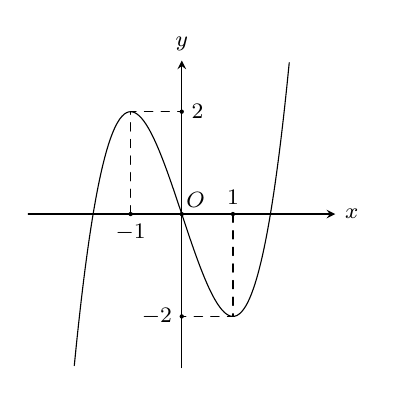
\begin{tikzpicture}[>=stealth,line join=round,line cap=round,font=\footnotesize,scale=0.65]
			\draw[->] (-3,0)--(3,0) node[right] {$x$};
			\draw[->] (0,-3)--(0,3) node[above] {$y$};
			\draw [smooth,domain=-2.1:2.1,samples=100]plot(\x,{(\x)^3-3*(\x)});
			\draw[dashed](-1,0)--(-1,2)--(0,2) (1,0)--(1,-2)--(0,-2);
			\fill (0,0)node[shift={(45:2.5mm)}]{\footnotesize{$O$}}circle(1.2pt) (1,0)node[above]{\footnotesize{$1$}}circle(1.2pt) (-1,0)node[below]{\footnotesize{$-1$}}circle(1.2pt) (0,2)node[right]{\footnotesize{$2$}}circle(1.2pt) (0,-2)node[left]{\footnotesize{$-2$}}circle(1.2pt);
		\end{tikzpicture}}
	\loigiai{
		\begin{itemchoice}
			\itemch Đồ thị hàm số có điểm cực đại là $(-1;2)$.
			\itemch Đồ thị hàm số cắt trục hoành $y=0$ tại ba điểm phân biệt.
			\itemch Đồ thị hàm số có hai điểm cực trị là $(-1;2)$ và $(1;-2)$ đối xứng với nhau qua gốc tọa độ $O$.
			\itemch Hàm số đồng biến trên $(-\infty;-1)$ và $(1;+\infty)$.
		\end{itemchoice}
	}
\end{ex}

\TNSA

\begin{ex}%[2D1V2-1]%[Dự án đề kiểm tra Toán GHKI NH 24-25- Đoàn Minh Tâm]%[THPT Phạm Văn Sáng - Tp HCM]
	Một vật chuyển động theo quy luật $s=-\dfrac{1}{4}t^{3}+6t^{2}$ với $t$ là khoảng thời gian tính từ khi vật bắt đầu chuyển động và $s$ (m) là quãng đường vật đi được trong khoảng thời gian đó. Biết trong khoảng thời gian $ 15 $ giây, kể từ khi bắt đầu chuyển động, vận tốc lớn nhất của vật đạt bằng bao nhiêu?
	\shortans[oly]{$ 48 $}
	\loigiai{
		Ta có $v(t)=s'(t)=-\dfrac{3}{4}t^2+12t $.\\
		Đề bài yêu cầu tìm giát trị lớn nhất của $ v(t) $ trên $ [0;15] $.\\
		Khi đó $ v'(t)= -\dfrac{3}{2}t+12$. Cho $ v'(t)=0 \Leftrightarrow -\dfrac{3}{2}t+12=0 \Leftrightarrow t=8 $.\\
		Ta tính được $ v(0)=0 $, $ v(8)= 48$, $ v(15)= 11{,}25$.\\
		Vậy vận tốc lớn nhất của vật đó là $ 48 $ m/s.
	}
\end{ex}

\begin{ex}%[2D1V2-2]%[Dự án đề kiểm tra Toán GHKI NH 24-25- Đoàn Minh Tâm]%[THPT Phạm Văn Sáng - Tp HCM]
	Một doanh nghiệp dự định sản xuất không quá $ 500 $ sản phẩm. Nếu doanh nghiệp sản xuất $x$ sản phẩm $(1 \le x \le 500)$ thì doanh thu nhận được khi bán hết số sản phẩm đó được biểu diễn bằng hàm là $F(x)=x^3-1\,999x^{2}+1\,001\,000x+250\,000$ (đồng), trong khi chi phí sản xuất bình quân cho một sản phẩm là  $G(x)=x+1\,000+\dfrac{250\,000}{x}$ (đồng). Doanh nghiệp cần sản xuất bao nhiêu sản phẩm để lợi nhuận thu được là lớn nhất?
	\shortans[oly]{	$ 250 $}
	\loigiai{
		Ta có $ x \in \mathbb{N} $ và $ 1 \le x \le 500 $.
		Ta có $F(x) = x^3-1\,999x^{2} + 1\,001\,000x + 250\,000$ và chi phí khi sản xuất $ x $ sản phẩm là $x\cdot G(x) = x^{2} + 1\,000x + 250\,000$.\\
		Gọi $ L(x) $ là hàm lợi nhuận, khi đó
		$$L(x) = F(x) - G(x) =x^3 -2\,000x^{2} + 1\,000\,000x \Rightarrow L'(x)=3x^2-4\,000x + 1\,000\,000.$$
		Ta cần tìm giá trị lớn nhất của $ F(x) $ trên $ [1;500] $.\\
		Cho $ L'(x)=0 \Leftrightarrow  3x^2-4\,000x + 1\,000\,000=0 \Leftrightarrow \hoac{&x=1\,000&\text{(loại)}\\&x=\dfrac{1\,000}{3}&\text{(nhận)}.}$\\
		Ta có bảng biến thiên như sau
		\begin{center}
			
\begin{tikzpicture}[>=stealth]
				\tkzTabInit[nocadre=true,lgt=2,espcl=3,deltacl=0.5]{$x$/1.5 ,$L'(x)$/.7,$L(x)$/2}
				{$1$ , $\dfrac{1\,000}{3}$ , $500$}
				\tkzTabLine{ , + , $0$ , - , }
				\tkzTabVar{-/$L(1)$ , +/$L\left(\dfrac{1\,000}{3}\right)$ , -/$L(500)$}
			\end{tikzpicture}
		\end{center}
		Do $ x $ là số tự nhiên nên ta xét $ L(333)= 146\,148\,037$ và $ L(334)= 148\,147\,704$.\\
		Vậy lợi nhuận lớn nhất khi sản xuất $ 333 $ sản phẩm.
	}
\end{ex}

\begin{ex}%[2D1V2-3]%[Dự án đề kiểm tra Toán GHKI NH 24-25- Đoàn Minh Tâm]%[THPT Phạm Văn Sáng - Tp HCM]
	Một tác giả muốn xuất bản một cuốn sách Toán học. Gọi $t $ ($t\ge 1$) là số cuốn sách sẽ in và tổng số tiền cần bỏ ra để in $t$ cuốn sách là $T=7\,000+50t$  (đơn vị nghìn đồng). Gọi $f(t)$ là chi phí trung bình cho mỗi cuốn sách. Khi số sách tăng lên thì chi phí trung bình của mỗi cuốn sách tối đa không vượt quá bao nhiêu nghìn đồng?
	\shortans[oly]{$ 50 $}
	\loigiai{
		Chi phí trung bình $f(t) = \dfrac{7\,000 + 50t}{t} = \dfrac{7\,000}{t} + 50$.\\
		Khi đó  $\lim\limits_{t\to +\infty} f(t) = 50$.\\
		Vậy chi phí trung bình không vượt quá $ 50 $ nghìn đồng.
	}
\end{ex}

\begin{ex}%[2D1V2-4]%[Dự án đề kiểm tra Toán GHKI NH 24-25- Đoàn Minh Tâm]%[THPT Phạm Văn Sáng - Tp HCM]
	Một xe khách đi từ TP.HCM đến Đà Nẵng chở tối đa được $ 60 $ hành khách mỗi chuyến. Nếu một chuyến chở được $m$ hành khách thì giá tiền cho mỗi hành khách được tính là $\left(300 - \dfrac{5m}{2}\right)^2$ đồng.	Tính số hành khách trên mỗi chuyến xe để nhà xe thu được lợi nhuận mỗi chuyến là lớn nhất?
	\shortans[oly]{$ 40 $}
	\loigiai{
		Doanh thu $
			R(m) = m\left(300 - \dfrac{5m}{2}\right)^2
			= 90\,000m -1\,500m^2+ \dfrac{25}{4}m^{3}$.
		Theo đề bài ta có điều kiện $ 0 \le m \le 60 $ và $ m\in \mathbb{N} $.\\
		Yêu cầu đề bài là tìm giá trị lớn nhất của $ R(m) $ trên $ [0;60] $.\\
		Ta có $	R'(m) = 90\,000 - 3\,000 m +\dfrac{75}{4}m^2$.\\
		Cho $ R'(m)=0 \Leftrightarrow 90\,000 - 3\,000 m +\dfrac{75}{4}m^2=0 \Leftrightarrow  \hoac{& x=120&\text{(loại)}\\&x=40&\text{(nhận)}.}$\\
		Ta có $ R(0)=0 $, $ R(40)= 1\,600\,000$, $ R(60)=1\,350\,000 $.\\
		Vậy chuyến xe thu lợi lớn nhất khi số hành khác là $ 40 $ hành khách.
	}
\end{ex}

\begin{ex}%[2D1V2-5]%[Dự án đề kiểm tra Toán GHKI NH 24-25- Đoàn Minh Tâm]%[THPT Phạm Văn Sáng - Tp HCM]
	Để giảm nhiệt độ phòng từ $28^\circ$C, một hệ thống làm mát được phép hoạt động trong $ 10 $ phút. Gọi $T$ (đơn vị $^\circ$C) là nhiệt độ phòng ở phút thứ $t$ được cho bởi công thức $T= - 0{,}008t^{3} - 0{,}16t + 28$ $(t \in [1;10])$. Tìm nhiệt độ thấp nhất trong phòng đạt được trong $ 10 $ phút kể từ khi hệ thống làm mát bắt đầu hoạt động.
	\shortans[oly]{$ 32{,}6 $	}
	\loigiai{
	Yêu cầu đề bài là tìm giá trị nhỏ nhất của $T(t) = -0{,}008t^{3} - 0{,}16t + 28$ trong $ [1;10] $.\\
	Ta có $	T'(t) = -0{,}024t^2 - 0{,}16 <0$, $ \forall t \in [0;10] $.\\
	Dẫn đến $ T $ là hàm nghịch biến trên $ [0;10] $.\\
	Vậy nhiệt độ thấp nhất là $T(10)= 18{,}4 ^\circ$C.
	}
\end{ex}

\begin{ex}%[2D1V2-6]%[Dự án đề kiểm tra Toán GHKI NH 24-25- Đoàn Minh Tâm]%[THPT Phạm Văn Sáng - Tp HCM]
	\immini[thm]{
		Công ty nước sạch Bình An đang cần lắp đặt đường ống dẫn nước từ nhà máy nước tới hòn đảo nhỏ trong sơ đồ (đường ống được xuất phát từ nhà máy đến điểm $T$ rồi đi ra đảo). Bến tàu cách đảo $ 1 $ km, đó chính là vị trí trên đất liền gần với đảo nhất. Nhà máy nước cách bờ biển $ 4 $ km. Biết rằng chi phí đặt một ki-lô-mét ống dẫn nước trên đất liền là $ 30 $ triệu đồng và còn lại đặt dưới nước là $ 50 $ triệu đồng. Khoảng cách từ điểm $T$ đến nhà máy nước là bao nhiêu ki-lô-mét để tổng chi phí lắp đặt là nhỏ nhất?}{
		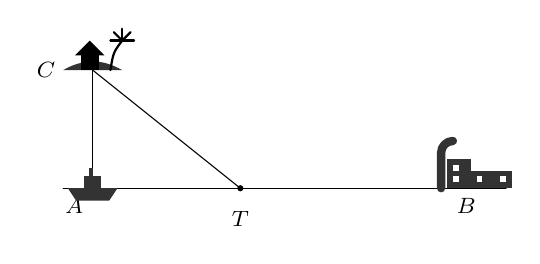
\begin{tikzpicture}[>=stealth,line join=round,line cap=round,font=\footnotesize,scale=0.75]

			% --- Định nghĩa toạ độ ---
			\coordinate (A) at (0,0);
			\coordinate (B) at (6,0); % Giả lập tỷ lệ ngang (4km)
			\coordinate (C) at (0,2); % Giả lập tỷ lệ đứng (1km) - vẽ cao hơn thực tế một chút để hình thoáng
			\coordinate (T) at (2.5,0); % Điểm T nằm giữa A và B

			% --- Vẽ các đường cơ bản ---
			% Đường bờ biển (AB) đậm
			\draw (-0.5,0) -- (7,0);

			% Đường từ đảo đến tàu (AC)
			\draw (C) -- (A);

			% Đường dây cáp/đường đi từ C đến T
			\draw (C) -- (T);

			% --- Vẽ các ký hiệu kích thước ---
			% Ký hiệu 1km (AC)
			%\node[left] at ($(A)!0.5!(C)$) {$ 1 $ km};

			% Ký hiệu 4km (AB) - cung tròn nét đứt bên dưới
			%\draw[dashed, <->] ($(A)+(0,-0.3)$) to[bend right=20] node[midway, below] {4 km} ($(B)+(0,-0.3)$);

			% Ký hiệu x (TB) - cung tròn nét đứt bên trên
			%\draw[dashed, <->] (T) to[bend left=45] node[midway, above] {$x$} (B);

			% --- Vẽ các điểm và nhãn ---
			\fill (T) circle (1.5pt) node[below=5pt] {$ T $};
			\node[below left] at (A) {$ A $};
			\node[below right] at (B) {$ B $};
			\node[left=10pt] at (C) {$ C $};

			% --- VẼ CÁC HÌNH MINH HOẠ (ICONS) ---

			% 1. Hòn đảo và ngôi nhà tại C
			\begin{scope}[shift={(C)}]
				% Đảo (đất)
				\fill[black!80] (-0.5,0) to[bend left=30] (0.5,0) -- cycle;
				% Ngôi nhà
				\fill[black] (-0.2,0) rectangle (0.1, 0.25);
				\fill[black] (-0.3,0.25) -- (-0.05,0.5) -- (0.2,0.25) -- cycle; % Mái nhà
				% Cây dừa
				\draw[thick, black] (0.3,0) .. controls (0.35,0.3) .. (0.5,0.5); % Thân
				\foreach \a in {0, 45, 90, 135, 180} {
						\draw[thick, black] (0.5,0.5) -- ++(\a:0.2); % Lá
					}
			\end{scope}

			% 2. Con tàu tại A
			\begin{scope}[shift={(A)}, scale=0.7]
				% Thân tàu
				\fill[black!80] (-0.6,0) -- (0.6,0) -- (0.4,-0.3) -- (-0.4,-0.3) -- cycle;
				% Cabin
				\fill[black!80] (-0.2,0) rectangle (0.2, 0.3);
				% Ống khói nhỏ
				\fill[black!80] (-0.1,0.3) rectangle (0, 0.5);
			\end{scope}

			% 3. Nhà máy tại B
			\begin{scope}[shift={(B)}]
				% Toà nhà chính
				\fill[black!80] (0,0) rectangle (0.4, 0.5);
				% Toà phụ
				\fill[black!80] (0.4,0) rectangle (0.8, 0.3);
				\fill[black!80] (0.8,0) rectangle (1.1, 0.3);
				% Cửa sổ (màu trắng)
				\foreach \x in {0.1, 0.5, 0.9}
				\fill[white] (\x, 0.1) rectangle ++(0.1,0.1);
				\fill[white] (0.1, 0.3) rectangle ++(0.1,0.1);

				% Ống khói cong (giống hình vẽ)
				\draw[line width=3pt, black!80] (-0.1,0) -- (-0.1,0.6) to[out=90, in=180] (0.1,0.8);
			\end{scope}

			% --- Trang trí thêm ---
			% Sóng nước dưới A
			%	\draw[decorate, decoration={snake, amplitude=1pt, segment length=5pt}] (-0.8,-0.4) -- (0.8,-0.4);

		\end{tikzpicture}
	}
	\shortans[oly]{$ 0{,}75 $}
	\loigiai{
	\begin{center}
		\begin{tikzpicture}[>=stealth,line join=round,line cap=round,font=\footnotesize,scale=0.75]

			% --- Định nghĩa toạ độ ---
			\coordinate (A) at (0,0);
			\coordinate (B) at (6,0); % Giả lập tỷ lệ ngang (4km)
			\coordinate (C) at (0,2); % Giả lập tỷ lệ đứng (1km) - vẽ cao hơn thực tế một chút để hình thoáng
			\coordinate (T) at (2.5,0); % Điểm T nằm giữa A và B

			% --- Vẽ các đường cơ bản ---
			% Đường bờ biển (AB) đậm
			\draw (-0.5,0) -- (7,0);

			% Đường từ đảo đến tàu (AC)
			\draw (C) -- (A);

			% Đường dây cáp/đường đi từ C đến T
			\draw (C) -- (T);

			% --- Vẽ các ký hiệu kích thước ---
			% Ký hiệu 1km (AC)
			\node[left] at ($(A)!0.5!(C)$) {$ 1 $ km};

			% Ký hiệu 4km (AB) - cung tròn nét đứt bên dưới
			\draw[dashed, <->] ($(A)+(0,-0.3)$) to[bend right=20] node[midway, below] {4 km} ($(B)+(0,-0.3)$);

			% Ký hiệu x (TB) - cung tròn nét đứt bên trên
			\draw[dashed, <->] (T) to[bend left=45] node[midway, above] {$x$} (B);

			% --- Vẽ các điểm và nhãn ---
			\fill (T) circle (1.5pt) node[below=5pt] {$ T $};
			\node[below left] at (A) {$ A $};
			\node[below right] at (B) {$ B $};
			\node[left=10pt] at (C) {$ C $};

			% --- VẼ CÁC HÌNH MINH HOẠ (ICONS) ---

			% 1. Hòn đảo và ngôi nhà tại C
			\begin{scope}[shift={(C)}]
				% Đảo (đất)
				\fill[black!80] (-0.5,0) to[bend left=30] (0.5,0) -- cycle;
				% Ngôi nhà
				\fill[black] (-0.2,0) rectangle (0.1, 0.25);
				\fill[black] (-0.3,0.25) -- (-0.05,0.5) -- (0.2,0.25) -- cycle; % Mái nhà
				% Cây dừa
				\draw[thick, black] (0.3,0) .. controls (0.35,0.3) .. (0.5,0.5); % Thân
				\foreach \a in {0, 45, 90, 135, 180} {
						\draw[thick, black] (0.5,0.5) -- ++(\a:0.2); % Lá
					}
			\end{scope}

			% 2. Con tàu tại A
			\begin{scope}[shift={(A)}, scale=0.7]
				% Thân tàu
				\fill[black!80] (-0.6,0) -- (0.6,0) -- (0.4,-0.3) -- (-0.4,-0.3) -- cycle;
				% Cabin
				\fill[black!80] (-0.2,0) rectangle (0.2, 0.3);
				% Ống khói nhỏ
				\fill[black!80] (-0.1,0.3) rectangle (0, 0.5);
			\end{scope}

			% 3. Nhà máy tại B
			\begin{scope}[shift={(B)}]
				% Toà nhà chính
				\fill[black!80] (0,0) rectangle (0.4, 0.5);
				% Toà phụ
				\fill[black!80] (0.4,0) rectangle (0.8, 0.3);
				\fill[black!80] (0.8,0) rectangle (1.1, 0.3);
				% Cửa sổ (màu trắng)
				\foreach \x in {0.1, 0.5, 0.9}
				\fill[white] (\x, 0.1) rectangle ++(0.1,0.1);
				\fill[white] (0.1, 0.3) rectangle ++(0.1,0.1);

				% Ống khói cong (giống hình vẽ)
				\draw[line width=3pt, black!80] (-0.1,0) -- (-0.1,0.6) to[out=90, in=180] (0.1,0.8);
			\end{scope}

			% --- Trang trí thêm ---
			% Sóng nước dưới A
			%	\draw[decorate, decoration={snake, amplitude=1pt, segment length=5pt}] (-0.8,-0.4) -- (0.8,-0.4);

		\end{tikzpicture}
	\end{center}
	Gọi $ BT=x $ (km) ($ 0<x<4 $).\\
	Chi phí $C(x)=30\cdot (4 - x) + 50\sqrt{x^{2}+1}=120 - 30x + 50\sqrt{x^{2}+1}$.\\
	Khi đó, ta có 	$C'(x)= -30 + \dfrac{50x}{\sqrt{x^{2}+1}}$.\\
	Cho $ C'(x)=0 \Leftrightarrow \dfrac{50x}{\sqrt{x^{2}+1}} = 30
		25x^{2} = 9(x^{2}+1) \Leftrightarrow 16x^{2} = 9 \Leftrightarrow	\hoac{&x=-0{,}75&\text{(nhận)}\\&x=0{,}75&\text{(nhận)}.}$\\
	Ta có bảng biến thiên như sau
	\begin{center}
		
\begin{tikzpicture}[>=stealth]
			\tkzTabInit[nocadre=true,lgt=2,espcl=3,deltacl=0.5]{$x$/.7 ,$C'(x)$/.7,$C(x)$/2}
			{$0$ , $0{,}75$ , $4$}
			\tkzTabLine{ , - , $0$ , + , }
			\tkzTabVar{+/$C(0)$ , -/$C(0{,}75)$ , +/$C(4)$}
		\end{tikzpicture}
	\end{center}
	Vậy khoảng cách từ điểm $ T $ đến nhà máy nước là $ 0{,}75 $ km để tổng chi phí là thấp nhất.
	}
\end{ex}

\Closesolutionfile{ans}
